Wir wollen nun eines der wichtigsten Werkzeuge f"ur die Analyse von diskreten \gls{lti}-Systemen einf"uhren und untersuchen.
Die $z$-Transformation nimmt f"ur diskrete \gls{lti}-Systeme dieselbe Rolle ein, wie die Laplace-Transformation f"ur zeitstetige \gls{lti}-Systeme.
Wir werden sehen, dass die Faltungs-Formel \eqref{eq:lti_sys:conv} im $z$-Bereich eine einfachere Form annimmt.
Au"serdem erlaubt uns die Transformation eine neue Sicht auf diskrete Systeme zu gewinnen, mit welcher es eventuell einfacher sein sollte gewisse Eigenschaften von Systemen nachzupr"ufen.
Wir werden auch sehen, dass sich manche Signale oder Systeme im $z$-Bereich kompakter aufschreiben lassen.

Die $z$-Transformation $X_\z: \C \rightarrow \C$ eines Signals $x[\cdot] : \N \rightarrow \C$ ist die komplexe Potenzreihe\linkfootnote{{https://mathworld.wolfram.com/LaurentSeries.html}}
\begin{equation}\label{eq:ztrafo:def}
    z \mapsto X_\z(z) = \Sum{n\in\Z}{}{x[n] z^{-n}}.
\end{equation}
Wegen der Summation "uber ganz $\Z$ ist $X_\z(z)$ f"ur jedes $z$ ein Grenzwert, der nicht existieren muss.
Das hei"st, es ist notwendig auch \emph{immer} den Konvergenzbereich, oder Englisch die \gls{roc}, von $X_\z$ anzugeben.

Betrachten wir beispielsweise \[x[\cdot] = \{5,6,\Start{3},4,-\pi\},\] dann ergibt sich \[X_\z(z) = 5 z^2 + 6 z + 3 + 4z^{-1} - \pi z^{-2} \Text{mit \gls{roc}} \C \setminus \{0\}.\] 
Im Fall von $x[\cdot] = \delta[\cdot-k]$, ergibt sich $X_\z(z) = z^{-k}$ mit \gls{roc} $\C \setminus \{0\}$, wobei sich bei $x[\cdot] = \delta[\cdot+k]$, sich $X_\z(z) = z^{k}$ mit \gls{roc} $\C$ ergibt.
Man sieht nun auch, weshalb das System, das ein Signal um einen Abtastwert verz"ogert, oft mit $z^{-1}$ bezeichnet wird, weil dies die $z$-Transformation dessen Impulsantwort ist.
Au"serdem kann man bei endlichen Signalen im $z$-Bereich deren Werte im Zeitbereich einfach ablesen. 
Will man den Wert $x[n]$, also an Sample $n$, ermittelt man diesen, indem man den Koeffizienten vom passenden $z^{-n}$ betrachtet. 

Aber auch f"ur unendlich lange Signale, wie beispielsweise $x[n] = a^n u[n]$, ergibt sich
\[
X_\z(z) 
    = 1 + a z^{-1} + a^2 z^{-2} + \dots
    = \Sum{n = 0}{\infty}{
        a^n z^{-n}
    }
    = \Sum{n = 0}{\infty}{
        \left(a z^{-1}\right)^n
    },
\]
was eine geometrische Reihe "uber $az^{-1}$ darstellt. 
Dann folgt, dass
\[
    X_\z(z) = \frac{1}{1 - a z^{-1}},
\]
wobei diese Potenzreihe nur konvergiert, wenn $z > a$.
Das hei"st, dass die \gls{roc} hier alle $z \in \C$ umfasst mit $\Abs{z} > \Abs{a}$.
Wir sehen, dass sich eigentlich unendlich lange Signale im $z$-Bereich durch Berechnen des Grenzwertes knapper darstellen lassen.
Gleichzeitig k"onnen wir so auch die \gls{roc} bestimmen, indem wir ermitteln, wann der ermittelte Grenzwert existiert.

Wenn wir $z = r\exp(\jmath \phi)$ in die Definition \eqref{eq:ztrafo:def} einsetzen und $\Abs{X_\z(z)}$ betrachten, finden wir
\[
\Abs{X_\z(z)} 
    = \Abs{\Sum{n\in\Z}{}{x[n] z^{-n}}}
    \leqslant \Sum{n\in\Z}{}{\Abs{x[n] z^{-n}}}
    = \Sum{n\in\Z}{}{\Abs{x[n] r^{-n}} \Abs{\exp(- \jmath n \phi)}}
    = \Sum{n\in\Z}{}{\Abs{x[n] r^{-n}}}.
\]
Betrachten wir den letzten Ausdruck genauer indem wir ihn in zwei Summationen aufteilen, also
\[
\Sum{n\in\Z}{}{\Abs{x[n] r^{-n}}} 
    = \Sum{n=-1}{-\infty}{\Abs{x[n] r^{-n}}}
    + \Sum{n=0}{+\infty}{\Abs{x[n] r^{-n}}}
    = \Sum{n=1}{+\infty}{\Abs{x[-n] r^{n}}}
    + \Sum{n=0}{+\infty}{\Abs{\frac{x[n]}{r^{n}}}}.
\]
Das ergibt dann also, dass
\[
    \Abs{X_\z(z)} 
        \leqslant \Sum{n=1}{+\infty}{\Abs{x[-n] r^{n}}}
        + \Sum{n=0}{+\infty}{\Abs{\frac{x[n]}{r^{n}}}}
\]
Damit $X_\z$ existiert, m"ussen beide Grenzwerte existieren.
Der erste Grenzwert existiert, wenn es ein $r_1$ gibt, sodass $r_1^n$ die Werte $x[-n]$ so gewichtet, das sich Konvergenz einstellt. 
Dieses $r_1$ ist ausschlie"slich durch die Werte in der \q{Vergangenheit} von $x[\cdot]$ bestimmt! 
Wenn sich Konvergenz f"ur ein $r_1$ einstellt, dann auch f"ur alle $r < r_1$.
Der Konvergenzbereich ergibt sich also als ein Kreis mit Radius $r_1$.
Der zweite Grenzwert existiert, falls f"ur ein $r_2 > 0$ die Werte $1/r_2^n$ so die \q{Zukunft} von $x[n]$ so wichten, dass die Summe konvergiert.
Das hei"st, falls so ein $r_2$ existiert, dann konvergiert der zweite Summand f"ur alle $r > r_2$.

Die \gls{roc} ist also die Schnittmenge von der Menge $\{\Abs{z} \leqslant r_1\}$ mit der Menge $\{\Abs{z} \geqslant r_2\}$.
Dies ist in \Cref{fig:ztrafo:roc} zusammengefasst. Wir sehen auch, dass im Falle von $r_1 > r_2$ die \gls{roc} die leere Menge ist und deshalb die $z$-Transformation nicht existiert.

\begin{figure}
    \centering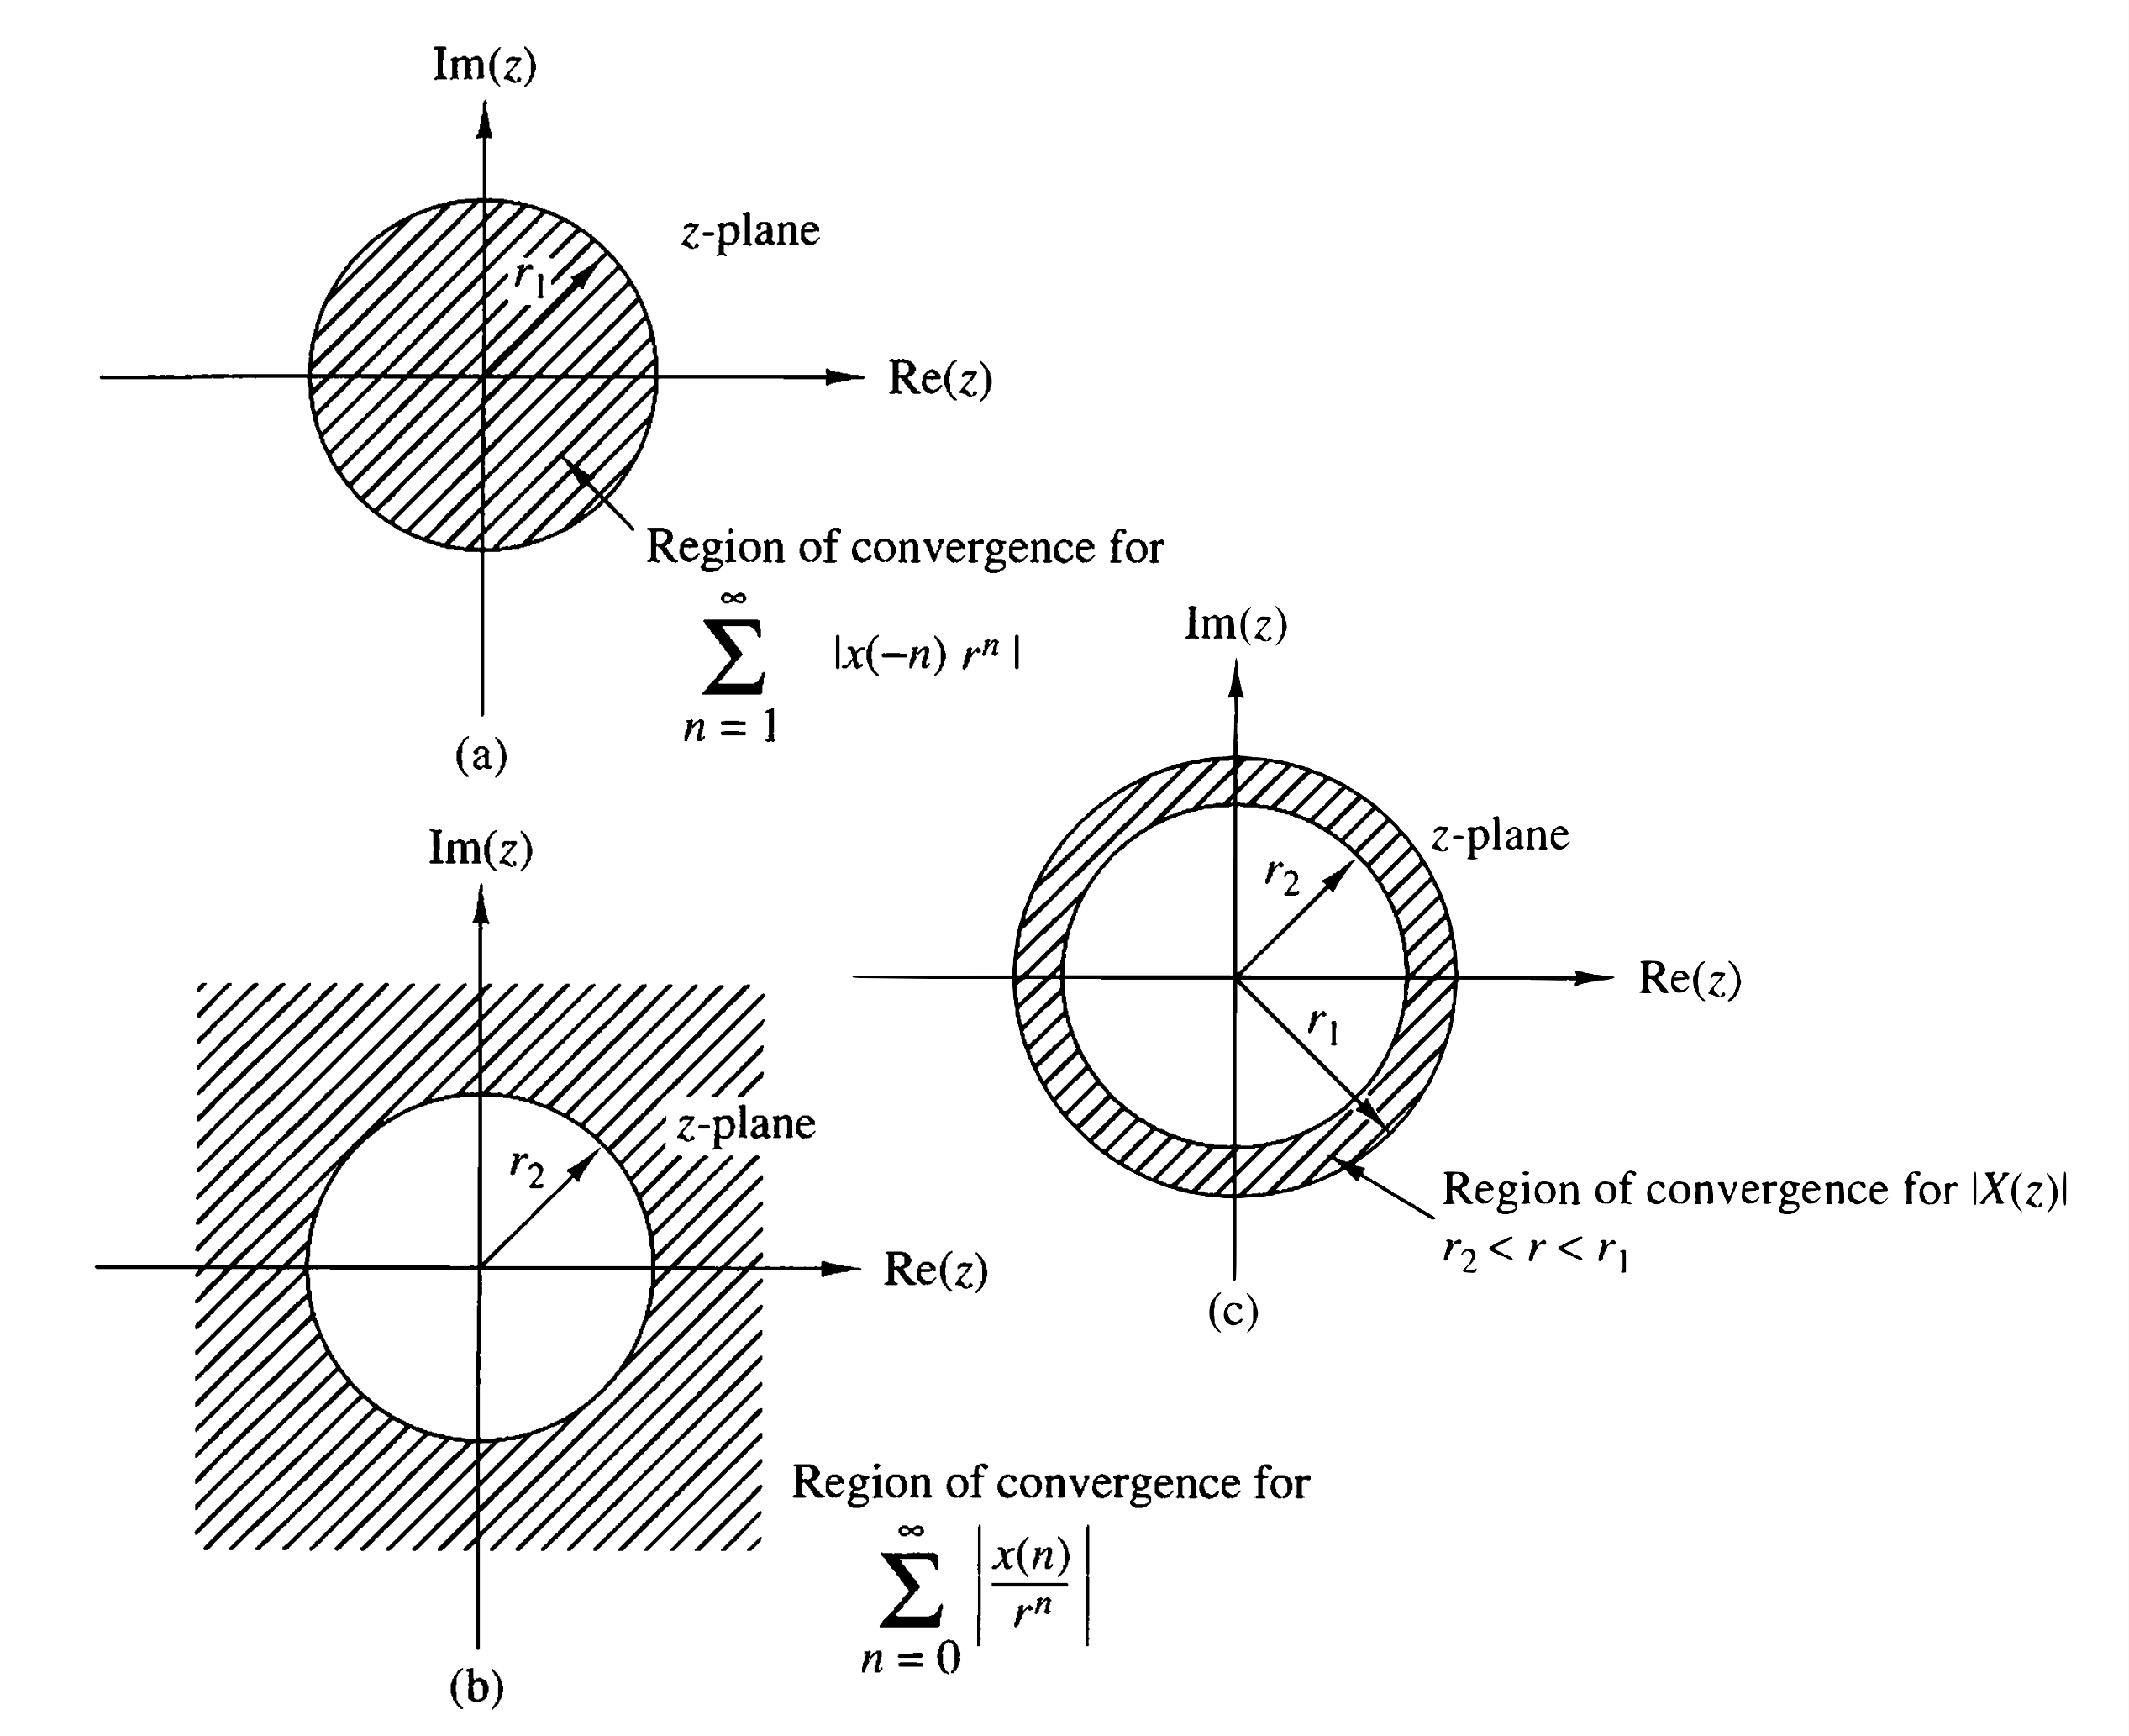
\includegraphics[width=0.8\textwidth]{img/ztrafo/roc.png}
    \caption{Veranschaulichung der Entstehung der \acrshort*{roc} aus den Konvergenzkriterien. Quelle: \cite{proakis2013}}\label{fig:ztrafo:roc}
\end{figure}
%
\subsubsection{Eigenschaften}\label{sec:ztrafo:properties}
%
Wir wollen nun einige Eigenschaften der $z$-Transformation auflisten, die wir immer wieder verwenden werden. 
Besonderes Augenmerk legen wir hierbei auf die Behandlung der \gls{roc}.
%
\paragraph{Linearit"at}
Gegeben zwei diskrete Signale $x_{1,2}[\cdot]$ und komplexe Zahlen $a_{1,2} \in \C$, dann gilt f"ur $x[\cdot] = a_1 x_1[\cdot] + a_2 x_2[\cdot]$, dass
\[
X_\z(z) = a_1 X_{\z,1}(z) + a_2 X_{\z, 2}(z),
\]
wobei die \gls{roc} von $X_{\z}$ der Schnittmenge der \glspl{roc} von $X_{\z,1}$ und $X_{\z,2}$ entspricht.
%
\paragraph{Zeitversatz}
Ist $X_\z$ die $z$-Transformation von $x[\cdot]$, so ist $z^{-k}X(z)$ die $z$-Transformation von $x[\cdot - k]$.
Hierbei ist die \gls{roc} von $X_{\z}$, falls $k\leqslant 0$.
Im Falle $k>0$ m"ussen wir aus der \gls{roc} von $X_{\z}$ den Wert $z=0$ entfernen.
Intuitiv sollte man diese Eigenschaft leicht verifizieren k"onnen, da man durch das Verschieben nur die Potenz des $z$ "andert und man diese "Anderung einfach ausklammern kann.

Um beispielsweise die $z$-Transformation von
\[
x[n] = \begin{cases}
    1, \Text{f"ur} 0 \leqslant n < N \\
    0 \Text{sonst}, 
\end{cases}
\]
zu bestimmen, k"onnten wir einerseits die Definition bem"uhen, oder die beiden schon bekannten Eigenschaften ausnutzen, um zu folgern, dass
\[
X_\z(z) = \begin{cases}
    N \Text{f"ur} z = 1,\\
    \frac{1 - z^{-N}}{1 - z^{-1}}
\end{cases}
\]
gilt.
Dazu nutzen wir, dass $x[n] = u[n] - u[n-N]$ gilt.
Da au"serdem $x[\cdot]$ nur endlich viele Werte verschieden von $0$ hat, ist die \gls{roc} von $X_\z$ die ganze $z$-Ebene, au"ser $z=0$.
%
\paragraph{Skalierung im \texorpdfstring{$z$}{z}-Bereich}
Ist $X_\z$ die $z$-Transformation von $x[\cdot]$ mit \gls{roc} $r_1 < \Abs{z} < r_2$, dann ist $a^n x[n]$ die inverse $z$-Transformation von $X(a^{-1} z)$ mit \gls{roc} $\Abs{a}r_1 < \Abs{z} < \Abs{a}r_2$.
Die Intuition hierbei ist, dass die Multiplikation mit der Folge $a^{n}$ mit $a=r\exp(\jmath \omega)$ eine Skalierung um $r$ und eine Rotation um $\omega$ im $z$-Bereich bewirkt.
Das hei"st gewisse \q{geometrische} Eigenschaften von $X_{\z}$ transformieren sich analog mit.
%
\paragraph{Zeitumkehrung}
Ist $X_\z$ die $z$-Transformation von $x[\cdot]$ mit \gls{roc} $r_1 < \Abs{z} < r_2$, dann ist $X_{\z}\left(z^{-1}\right)$ die $z$-Transformation von $x[-\cdot]$ mit \gls{roc} $1/r_1 < \Abs{z} < 1/r_2$.
Mit anderen Worten entspricht Umkehrung im Zeitbereich Reflexion am Einheitskreis im $z$-Bereich.
%
\paragraph{Faltung im Zeitbereich}
%
Kommen wir nun zu einer der wichtigsten Eigenschaften und einem der Gr"unde, weshalb die $z$-Transformation als Analogie zur Laplace-Transformation verstanden wird.
Gegeben zwei diskrete Signale $x_{1,2}[\cdot]$ und $x[\cdot] = x_1 \ast x_2$, dann gilt 
\begin{equation}\label{eq:ztrafo:conv}
    X_{\z}(z) = X_{\z,1}(z) \cdot X_{\z,2}(z),
\end{equation}
wobei die \gls{roc} mindestens die Schnittmenge der \glspl{roc} von $X_{\z,1}(z)$ und $X_{\z,2}(z)$ ist.
Der Grund f"ur das \q{mindestens} ist die Tatsache, dass f"ur gewisse $z$ die Divergenz von $X_{\z,1}$ durch rasches Tendieren von $X_{\z,2}$ gegen $0$ kompensiert werden kann.

Wegen ihrer Bedeutung, wollen wir uns kurz "uberlegen, warum die obige Eigenschaft gilt.
Wir nutzen im Grunde nur die Definition \eqref{eq:ztrafo:def} und die Definition der Faltung, um zu sehen, dass
\[
X_\z(z) 
    = \Sum{n \in \Z}{}{x[n] z^{-n}} 
    = \Sum{n \in \Z}{}{
        \Sum{k \in \Z}{}{x_1[k] x_2[n - k]} z^{-n}
      } 
    = \Sum{k \in \Z}{}{
        x_1[k] \Sum{n \in \Z}{}{x_2[n - k]} z^{-n}
    }.
\]
Jetzt nutzen wir die Eigenschaft, die sich aus dem Zeitversatz gibt zusammen mit \eqref{eq:ztrafo:def}, und erhalten schlussendlich
\[
    X_\z(z) 
    = \Sum{k \in \Z}{}{
        x_1[k] \Sum{n \in \Z}{}{x_2[n - k]} z^{-n}
    } 
    = \Sum{k \in \Z}{}{
        x_1[k] X_{\z, 2}(z) z^{-k}
    }
    = X_{\z, 2}(z) \Sum{k \in \Z}{}{
        x_1[k] z^{-k}
    }
    = X_{\z,1}(z) X_{\z, 2}(z).
\]
Wir k"onnen also zusammenfassend folgende Herangehensweise bei der Berechnung der Faltung angeben:
\begin{enumerate}
    \item Transformation von $x_{1,2}[\cdot]$ zu $X_{\z,1,2}$
    \item Punkweise Multiplikation von $X_{\z}(z) = X_{\z,1}(z) X_{\z,2}(z)$
    \item R"ucktransformation von $X_{\z}(z)$ zu $x[\cdot] = x_1 \ast x_2$
\end{enumerate}
%
\paragraph{Inverse \texorpdfstring{$z$}{z}-Transformation}
Obige Berechnung der Faltung verlangt im letzten Schritt die Invertierung der $z$-Transformation von $X_{\z}$ zu $x[\cdot]$.
Im allgemeinen Fall ist man darauf angewiesen den Cauchyschen Integralsatz~\linkfootnote{{https://de.wikipedia.org/wiki/Cauchyscher_Integralsatz}} zu bem"uhen.
Am Ende erlaubt dieser die Herleitung von
\begin{equation}\label{eq:ztrafo:inv}
    x[n] = \frac{1}{\jmath 2 \pi} \ointctrclockwise\limits_{C \subset \mathrm{ROC}} X_{\z}(z) z^{n-1} \mathrm{d}z
\end{equation}
als M"oglichkeit der Bestimmung von $x[n]$ aus $X_{\z}$.
Oft sind diese Integrale jedoch nicht leicht zu Berechnen und man sollte sich auf geeignete Tabellen (siehe~\cite[Tabelle~3.2,~Tabelle~3.3]{proakis2013}) und die restlichen obigen Eigenschaften beziehen, wenn man $z$-Transformationspaare bestimmen m"ochte.
%
%
\subsubsection{Anwendung bei diskreten \texorpdfstring{\acrshort*{lti}}{LTI}-Systemen}
%
Wir kombinieren nun \eqref{eq:lti_sys:conv} mit \eqref{eq:ztrafo:conv}, um eine alternative Beschreibung von \gls{lti}-Systemen zu erhalten.
Wir wissen aus \eqref{eq:lti_sys:conv}, dass sich das Eingabe-Ausgabe-Verhalten von einem \gls{lti}-System $\mathcal{T}$ durch
\[
y[\cdot] = h \ast x
\]
ausdr"ucken l"asst, wobei $h[\cdot] = y[\cdot]$ f"ur $x[\cdot]=\delta$.
Im $z$-Bereich transformiert sich dies wegen \eqref{eq:ztrafo:conv} zu
\begin{equation}\label{eq:ztrafo:transfer_function}
    Y_\z(z) = H_\z(z) X_\z(z).
\end{equation}
Man nennt dann $H_{\z}$ als $z$-Transformation der Impulsantwort die \emph{Transferfunktion} des Systems $\mathcal{T}$.
Wir haben so eine alternative Sichtweise auf \gls{lti}-Systeme gewonnen, weil man eben durch die $z$-Transformation die Impulsantwort $h[\cdot]$ mit der Transferfunktion $H$ \emph{identifiziert}.
Das hei"st, dass beide Beschreibungen "aquivalent sind.
Wir werden uns wie in \Cref{sec:lti_sys:properties} "uberlegen, wie man gewissen Eigenschaften von \gls{lti}-Systemen an $H$ \q{ablesen} kann.

Aus diesem multiplikativen Zusammenhang kann man bei Kenntnis von zwei Gr"o"sen in der Regel die fehlende Dritte bestimmen.
Kennt man beispielsweise $H_\z$ und $X_\z$, dann kann man sehr einfach $Y_\z$ und damit auch $y[\cdot]$ bestimmen.
In bestimmten Anwendungen der Messtechnik ist man eher daran interessiert durch geschickte Messungen $h[\cdot]$ zu bestimmen.
Dies kann unter anderem interessant sein, wenn in $h[\cdot]$ gewisse Parameter eines Systems \q{versteckt} sind, die einen aber interessieren.
Dann ist es oft geschickt das System durch $x[\cdot]$ anzuregen, $y[\cdot]$ zu beobachten und dann die Transferfunktion durch
\[
H_\z(z) = \frac{Y_\z(z)}{X_\z(z)}
\]
zu bestimmen.
Man muss sich im Klaren hierbei sein, dass es hierzu notwendig ist das Signal $x[\cdot]$ so zu w"ahlen, dass obige Division ein hinreichend genaues Bild von $h[\cdot]$ erlaubt.
%
%
\paragraph{Rekursive Systeme}
Ist allgemein die Vorschrift von einem System gegeben durch
\[
y[n] = -\Sum{k=1}{N}{a_k y[n-k]} + \Sum{k=0}{M}{b_k x[n - k]},
\]
dann ergibt sich durch die Linearit"at, Zeitversatz und geschicktes Umstellen, dass
\[
    H(z) = \frac{\Sum{k=0}{M}{b_k z^{-k}}}{1 + \Sum{k=1}{N}{a_k z^{-k}}}.
\]
Das hei"st, dass Systeme, die durch lineare Differenzengleichungen charakterisiert sind, besitzen eine Transferfunktion, die die Struktur einer rationalen Funktion
\[
H_\z(z) = \frac{B(z)}{A(z)}
\]
hat, wenn wir fordern, dass $A$ und $B$ Polynome in $z$ sind.
Allgemein schreiben wir
\[
H(z) = 
    \frac{
        b_0 + b_1 z^{-1} + \dots + b_M z^{-M}
    }{
        a_0 + a_1 z^{-1} + \dots + a_N z^{-N}
    }
    = \frac{
        \Sum{k = 1}{M}{b_k z^{-k}}
    }{
        \Sum{k = 1}{N}{a_k z^{-k}}
    }
    = G z^{N - M} \frac{
        (z - z_1) \dots (z - z_M)
    }{
        (z - p_1) \dots (z - p_N)
    }.
\]
Dann nennen wir die $z_1, \dots, z_M$ die \q{Nullstellen}, oder \emph{zeros}, des Systems $\mathcal{T}$ und die Menge $p_1 ,\dots, p_N$ die \emph{Pole}, oder \emph{Polstellen}, von $\mathcal{T}$.
Tritt ein $p_i$ oder $z_i$ mehrfach auf, so sprechen wir von einer mehrfachen Polstelle, bzw.\,Nullstelle.
Die Anzahl an gleichen Null-/Polstellen nennt man ihre Vielfachheit.

Es gibt nun zwei Spezialf"alle, die wir betrachten k"onnen. 
Erstens, es gilt $a_1 = \dots = a_N = 0$. 
In diesem Fall gilt 
\[
H(z) = z^{-M} \Sum{k = 1}{M}{b_k z^{M-k}}
\]
und $H$ besitzt als Polynom vom Grad $M$ dann $M$ Nullstellen~\linkfootnote{{https://de.wikipedia.org/wiki/Fundamentalsatz_der_Algebra}} und eine $M$-fache Polstelle bei $z=0$.
Tritt eine Polstelle bei $z=0$ auf, so nennen wir diese \emph{trivial}, da sie keinen Einfluss auf das System hat.
Schlie"slich korrespondiert $z^{-M}$ nur zu einer Verschiebung im Zeitbereicht, was bei \gls{lti}-Systemen per definitionem nur eine globale Verschiebung der ganzen Systems bedeutet.
Da keine nicht-trivialen Polstellen auftreten, hat das System eine \emph{endliche} Impulsantwort.
Das k"onnen wir daran sehen, dass wir die Werte von $h[\cdot]$ direkt an den Koeffizienten von $H$ ablesbar sind.

Zweitens, kann es vorkommen, dass $b_1 = \dots = b_N = 0$, was wiederum $H$ zu einer rationalen Funktion macht, die keine Nullstellen und dementsprechend ausschlie"slich Polstellen besitzt.
Um zu bestimmen, welche Implikation dies hat, betrachten wir ein einfaches System mit einem reellen Pol bei $a \in \R$, also
\[
H(z) = \frac{1}{1 - a z^{-1}}, ROC: \Abs{z} > \Abs{a}.
\]
Wie wir weiter oben schon gesehen haben, ist die zugeh"orige Impulsantwort $h[\cdot]$ gegeben durch
\[
h[n] = a^n u[n].
\]
%
\begin{figure}
    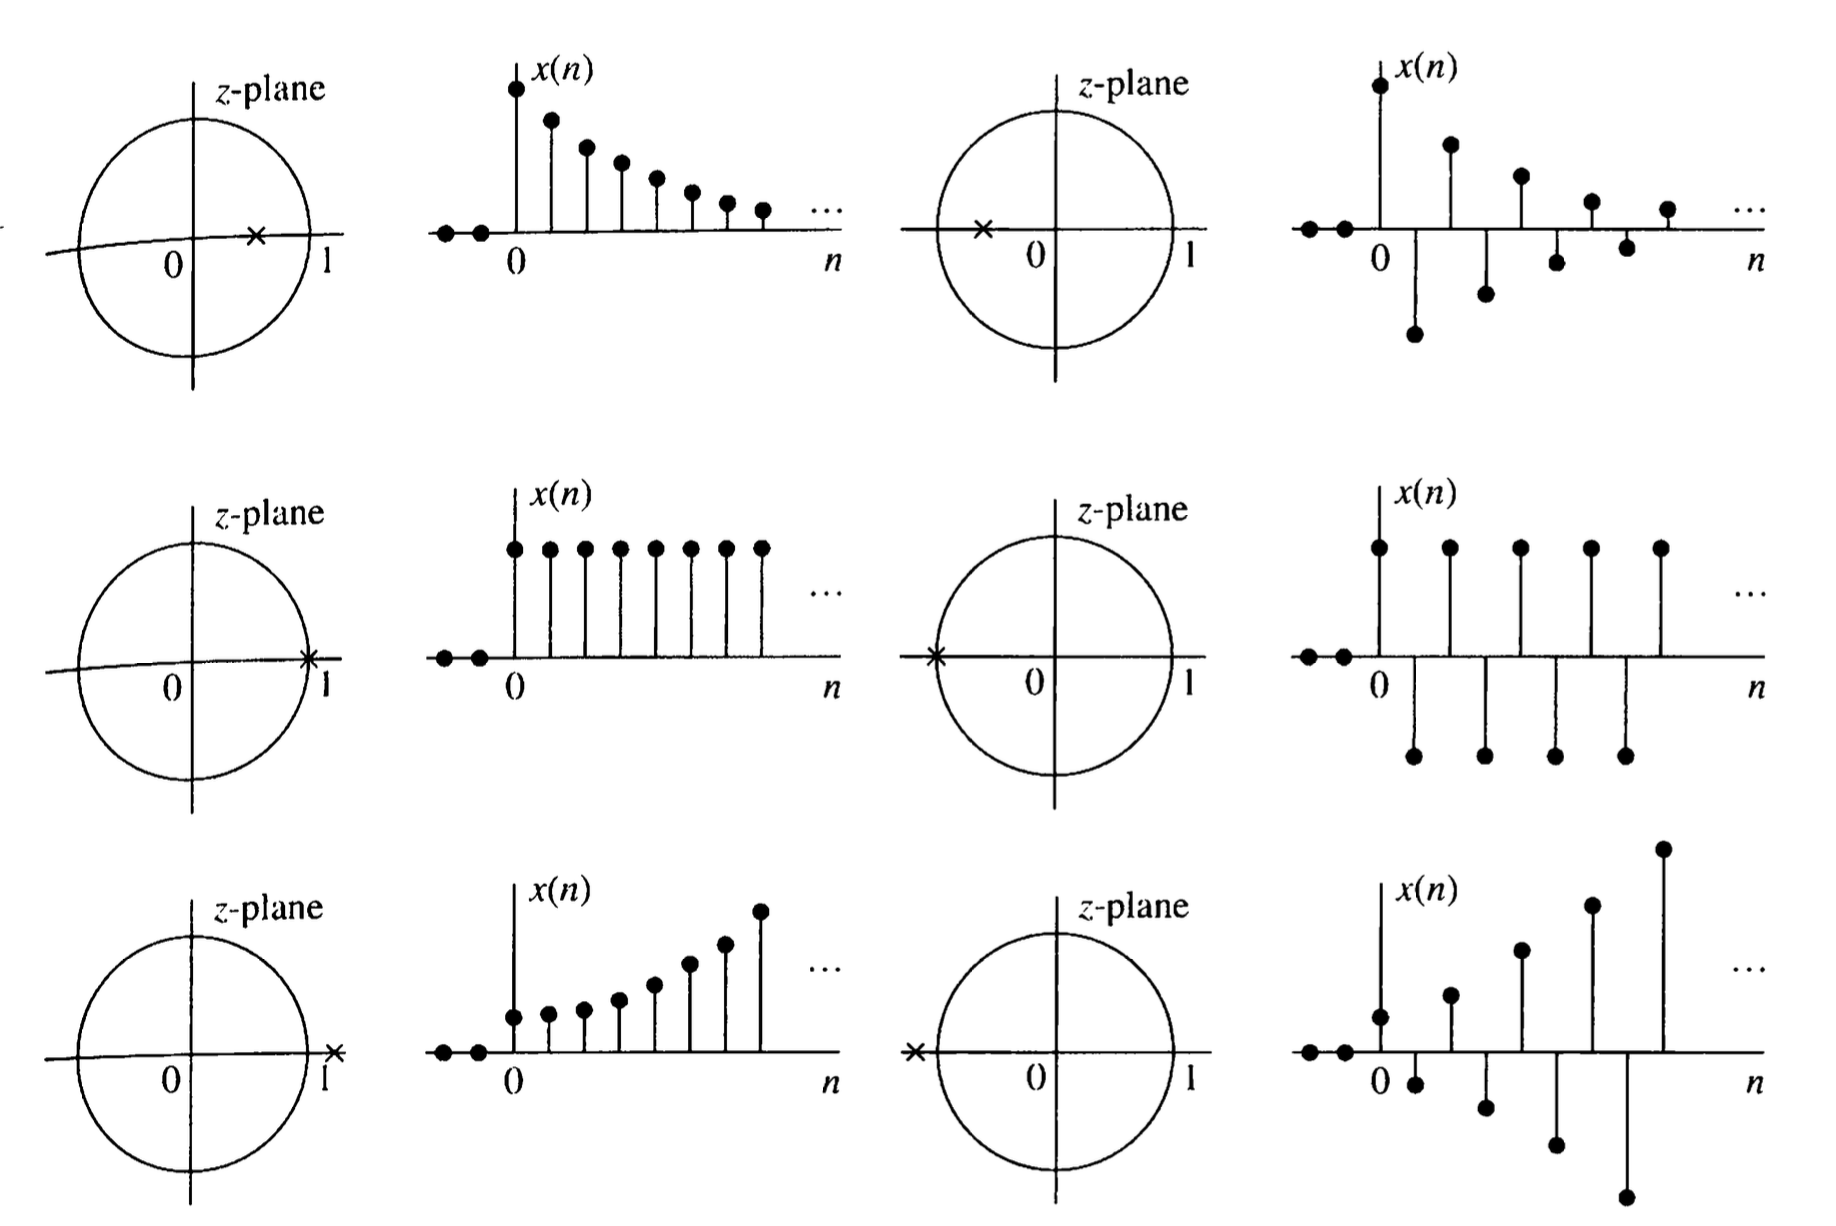
\includegraphics[width=0.9\textwidth]{img/ztrafo/singlepole.png}
    \caption{Impulsantwort $h[n] = a^n u[n]$ f"ur verschiedene Werte von $a$, Quelle: \cite{proakis2013}}\label{fig:ztrafo:singlepole}
\end{figure}

Das Verhalten von diesem System ist in \cref{fig:ztrafo:singlepole} dargestellt.
Man sieht, dass der Einheitskreis in der komplexen Ebene eine entscheidende Rolle spielt.
Liegt $a$ innerhalb des Einheitskreises, so ergibt sich eine exponentiell abfallende Impulsantwort.
Falls $a < 0$, stellt sich auch eine Oszillation ein.
F"ur $\Abs{a} = 1$ entspricht der Betrag der Impulsantwort der Heavyside-Funktion $u[\cdot]$.
Man sieht, dass im Fall von $\Abs{a} < 1$ die Impulsantwort absolut summierbar ist, also
\[
\Sum{n \in \Z}{}{\Abs{h[n]}} < \infty,
\]
was impliziert, dass das System stabil ist.
Entsprechend, ist das System instabil, falls $\Abs{a} > 1$.
Man sieht also, dass die Position der Pole im $z$-Bereich direkt interpretierbar ist.
Betrachtet man nochmals die \gls{roc} $\Abs{z} > \Abs{a}$, zusammen mit der Information, dass sich Stabilit"at einstellt, falls $\Abs{a}<1$.
Geometrisch bedeutet dies, dass das System stabil ist, falls der Einheitskreis in der \gls{roc} enthalten ist.

Diese Resultate lassen sich auf mehrere Polstellen verallgemeinern, da $H$ nur mehr Pole enth"alt und die \gls{roc} dann sich nach dem Betrag der \q{gr"o"sten} Polstelle richtet.
Das hei"st ultimativ, dass sich f"ur ein System $H$ Stabilit"at einstellt, falls \emph{alle} Polstellen sich im Einheitskreis befinden, \emph{oder} "aquivalent, dass sich der Einheitskreis in der \gls{roc} befinden muss.
Sp"ater werden wir noch eine Bedingung f"ur Stabilit"at in Bezug auf die Fourier-Transformation finden.
